\chapter{Background}
\label{chap:background}


The Keystone framework is built on the RISC-V instruction set architecture, which provides a unique foundation for secure system design due to its open specification and modular extensibility. Unlike traditional ISAs that are controlled by single vendors, RISC-V encourages community-driven enhancements and supports custom extensions, making it particularly attractive for trusted computing research and development. Its clean and well-documented privilege model allows for the implementation of isolation mechanisms that are critical to the construction of TEEs.

RISC-V defines three primary privilege levels: user mode (U-mode), supervisor mode (S-mode), and machine mode (M-mode). These privilege levels are hierarchical, with M-mode having the highest authority over system resources. M-mode has direct access to all hardware features and is responsible for critical functions such as interrupt control, exception handling, and access to physical memory protection mechanisms. Keystone leverages this privilege model by placing its Security Monitor (SM)—the core of the TCB—in M-mode. The SM is responsible for managing enclaves, enforcing memory isolation, and mediating access to sensitive system operations. By situating the TCB in M-mode, Keystone ensures that enclave isolation policies are enforced at the highest level of privilege, thereby minimizing the attack surface.

A central hardware feature used by Keystone is Physical Memory Protection (PMP), introduced in version 1.10 of the RISC-V Privilege Specification. PMP enables M-mode software to define access permissions for specific physical memory regions, controlling which lower-privilege modes (U and S) may read, write, or execute code in those regions. This capability forms the basis of Keystone’s memory isolation model. Each enclave is allocated a private memory region protected by PMP, ensuring that neither the host operating system nor any unauthorized software can access its contents. PMP rules are enforced directly by hardware, providing strong guarantees of isolation that are resistant to software-based attacks.

In addition to memory protection, RISC-V supports a flexible trap and exception handling mechanism. M-mode can intercept and handle all traps, but may delegate certain classes of exceptions—such as system calls and page faults—to S-mode for performance optimization. This delegation allows the enclave runtime to cooperate with the host operating system for memory management tasks, while still maintaining strict control over enclave boundaries. The virtual memory subsystem is managed through the standard RISC-V MMU, which translates virtual addresses to physical addresses using multi-level page tables. Keystone leverages this infrastructure to support enclaves that operate with their own private address spaces, protected by PMP from tampering or inspection.

Importantly, the use of standard programming models and toolchains for M-mode software development makes the Keystone Security Monitor both maintainable and extensible. Unlike microcode or hardwired logic, which are difficult to audit and update, the SM is implemented in C and can be subjected to conventional testing and formal verification techniques. This increases the transparency and trustworthiness of the TCB, which is a critical requirement for secure system design.

Taken together, the combination of RISC-V’s privilege hierarchy, PMP, trap delegation mechanisms, and extensibility provides a solid foundation for implementing robust and configurable TEEs. The Keystone framework capitalizes on these features to deliver a flexible and open platform for secure enclave execution, while remaining faithful to the RISC-V philosophy of openness and modularity.

\section{Trusted Execution Environments}
Trusted Execution Environments (TEEs) represent a class of hardware-assisted secure computing technologies that provide strong guarantees for the confidentiality and integrity of both code and data, even in systems where the underlying operating system or application software may be compromised. TEEs are designed to protect sensitive computations from a wide range of adversaries by establishing isolated execution contexts—commonly referred to as enclaves—through a combination of hardware features and privileged system software.

A TEE isolates a subset of the system’s resources, including CPU registers, memory, and I/O peripherals, and makes them accessible only to trusted applications executing within the enclave boundary. This isolation is enforced by the processor’s privilege mechanisms, memory protection units, or dedicated security monitors, ensuring that unauthorized entities—whether kernel-level malware or user-space processes—cannot access or tamper with enclave-resident assets.

Security within a TEE is achieved by reducing the size and complexity of the Trusted Computing Base (TCB). The TCB encompasses the set of components that must be trusted for the TEE to function securely. A minimal TCB is desirable, as it reduces the likelihood of vulnerabilities and simplifies formal verification and auditing processes. Modern TEEs aim to move as few components as possible into the TCB, while still providing robust isolation and essential services.

Prominent commercial TEE implementations include Intel Software Guard Extensions (SGX) and ARM TrustZone. Intel SGX facilitates the creation of enclaves at the user level, with memory encryption and access control enforced by hardware. ARM TrustZone, in contrast, provides a split-world architecture that partitions the processor into a secure world and a normal world, with secure world execution isolated via monitor calls. While these solutions have been successfully deployed in many real-world systems, their proprietary nature, rigid designs, and opaque implementations inhibit their utility for research, experimentation, and system-level innovation.

In response to these limitations, open-source TEE frameworks such as Keystone have emerged. Keystone is built atop the RISC-V instruction set architecture (ISA), which is itself open, extensible, and amenable to security-centric innovation. RISC-V’s modularity enables the design of TEEs that are both highly customizable and more transparent in their operation. A foundational architectural principle shared by all TEEs, including Keystone, is privilege separation. This concept involves executing the core TCB in a highly privileged execution mode—such as machine mode (M-mode) in RISC-V—while relegating the operating system and general-purpose applications to less privileged levels. This separation is crucial for enforcing isolation policies and preventing untrusted software from influencing the secure execution environment.

By leveraging privilege separation, physical memory protection, and modular TCB design, TEEs provide a powerful framework for secure computation in adversarial environments. Keystone builds upon these principles and extends them with openness and configurability, making it a valuable platform for academic and practical exploration of TEE technologies.

\section{Keystone Architecture Overview}

Keystone is an open-source Trusted Execution Environment (TEE) framework built on the RISC-V architecture, designed to enable customizable, lightweight, and secure enclaves suitable for both research and deployment in resource-constrained or security-critical settings \cite{dayeol2019keystone}. The framework’s modular design emphasizes a minimal Trusted Computing Base (TCB), portability across diverse RISC-V platforms, and extensibility to accommodate advanced security features, reflecting a clean and flexible architectural philosophy.

Keystone leverages the multiple privilege modes defined by the RISC-V specification—user mode (U-mode), supervisor mode (S-mode), and machine mode (M-mode)—to enforce security policies effectively. At the core of Keystone’s TCB is the Security Monitor (SM), which executes in M-mode and holds exclusive authority over enclave lifecycle management, memory protection configuration, and access control enforcement. The SM uses RISC-V’s Physical Memory Protection (PMP) mechanism to isolate enclave memory regions dynamically, ensuring strict access controls during enclave execution \cite{dayeol2019keystone}.

A typical Keystone-enabled platform comprises RISC-V cores augmented with secure boot mechanisms, trusted entropy sources, and optionally, hardware accelerators for cryptographic functions or secure I/O. Importantly, Keystone does not require hardware beyond standard RISC-V compliance and PMP support, making it adaptable to implementations ranging from FPGA prototypes to silicon SoCs \cite{dayeol2019keystone}.

Each enclave in Keystone consists of two main software components: a user-level enclave application (eapp) containing application-specific logic, and a supervisor-level runtime (RT) providing essential operating system abstractions such as exception handling, system call services, and memory management. This layered approach reduces the complexity of enclave applications and provides a trusted runtime environment isolated from the untrusted operating system and other processes \cite{dayeol2019keystone}.

The enclave lifecycle is structured into three primary phases: creation, execution, and destruction. During creation, the SM validates and locks the enclave’s memory layout—referred to as Enclave Page Memory (EPM)—with PMP to ensure confidentiality and integrity. During execution, the SM mediates context switches between the host and enclave, dynamically adjusting PMP to maintain isolation. Destruction securely erases enclave memory to prevent any residual data leakage \cite{dayeol2019keystone}. Keystone also supports optional features such as remote attestation, allowing external verifiers to authenticate enclave state prior to provisioning sensitive data, and can be extended for secure I/O and cryptographic acceleration.

\begin{figure}[htbp]
\centering
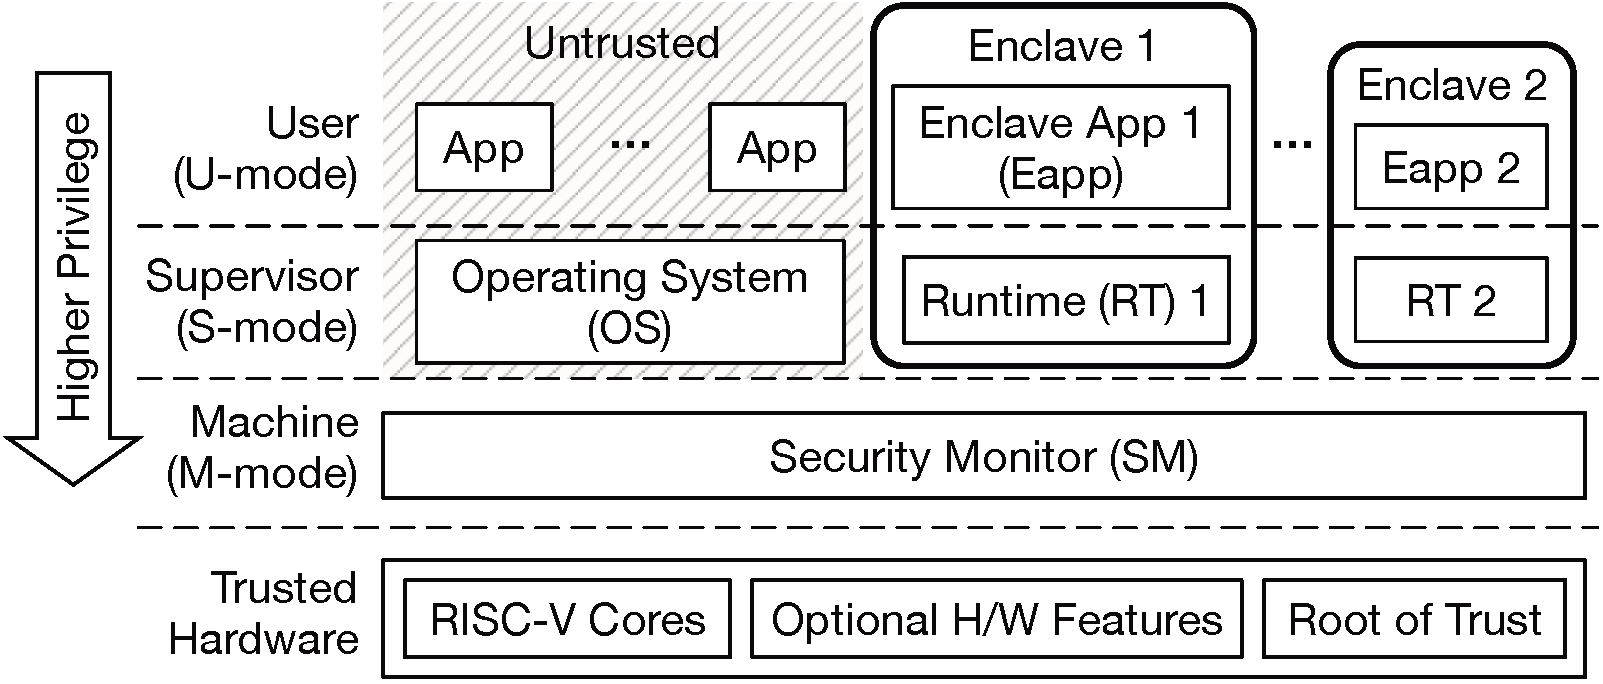
\includegraphics[width=0.9\linewidth]{figures/keystone_overview.png}
\caption{Overview of the Keystone architecture illustrating components such as the Security Monitor, enclave runtime, and the privilege hierarchy.}
\label{fig:keystone_overview}
\end{figure}

\begin{figure}[htbp]
\centering
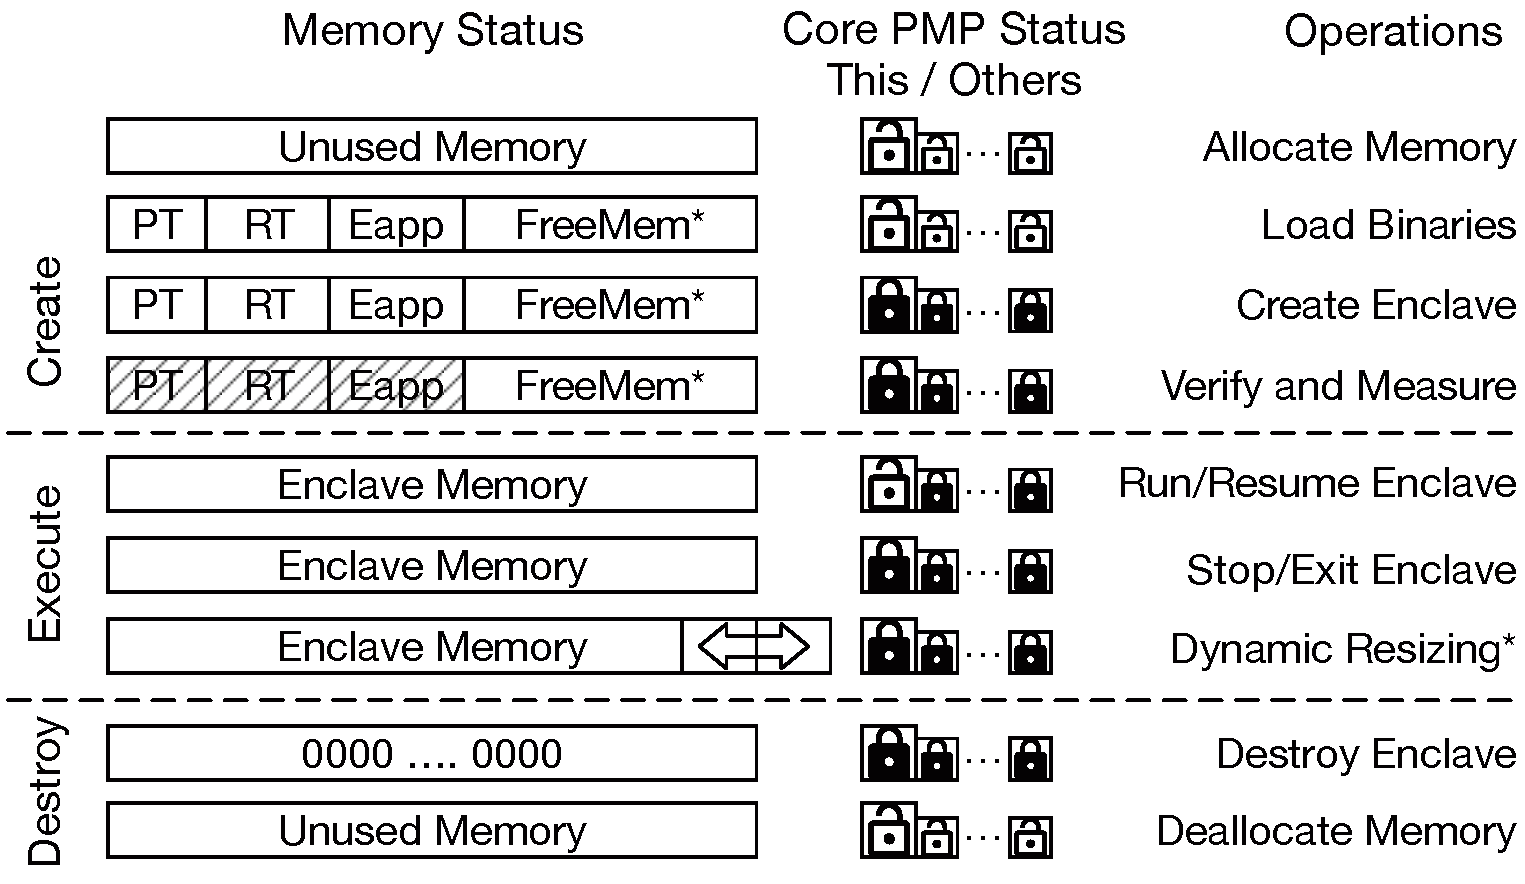
\includegraphics[width=0.9\linewidth]{figures/enclave_lifecycle.png}
\caption{Stages of a Keystone enclave lifecycle: creation, execution, and destruction.}
\label{fig:enclave_lifecycle}
\end{figure}

Overall, Keystone’s modular and open framework leverages the openness of RISC-V to provide strong security guarantees while enabling flexibility for research and customization. Its minimal TCB, modular layering (Security Monitor, runtime, eapp), and standards-compliant interfaces make it an attractive platform for developing and evaluating secure applications on modern processors \cite{dayeol2019keystone}.

\section{Kyber: A Post-Quantum Cryptography Algorithm}

\section{Comparison with Other TEEs}

Keystone’s architecture sets it apart from existing commercial Trusted Execution Environments such as Intel Software Guard Extensions (SGX) and ARM TrustZone through its openness, modularity, and alignment with the RISC-V ecosystem \cite{dayeol2019keystone}. Unlike the proprietary and largely opaque designs of SGX and TrustZone, Keystone offers a fully open-source platform that supports fine-grained system-level customization and experimental research.

ARM TrustZone implements a dual-world execution model that partitions the processor into a Secure World and a Normal World, with transitions managed via secure monitor calls (SMCs). While TrustZone provides a trusted OS environment (e.g., OP-TEE) within the Secure World, it supports only a single secure instance and requires significant overhead for context switches and interrupt handling. Moreover, the TrustZone TCB encompasses the entire Secure World kernel and trusted services, which increases complexity and hinders formal verification \cite{dayeol2019keystone}.

Intel SGX allows dynamic creation of enclaves at runtime within user-mode processes and provides memory encryption to isolate enclave data from the OS and hypervisor. However, SGX enclaves are confined to user mode and cannot run supervisor-level code, limiting their expressiveness. Additionally, SGX enforces rigid constraints on enclave size and structure, and its reliance on Intel hardware restricts portability and adaptability \cite{dayeol2019keystone}.

Keystone synthesizes the advantages of both approaches while overcoming their limitations. It supports dynamic enclave creation and hierarchical privilege separation by utilizing both user and supervisor modes, controlled by a minimal M-mode Security Monitor. The use of PMP allows Keystone to enforce spatial and temporal memory isolation without the complexity of encryption or hardware-bound restrictions \cite{dayeol2019keystone}.

Communication between the host and enclaves is facilitated by a lightweight interface named keyedger, akin to SGX’s edger8r but designed for greater flexibility and extensibility. Keystone partially supports the GlobalPlatform TEE Internal API and is architected to accommodate custom APIs, enhancing its utility for diverse research and deployment scenarios \cite{dayeol2019keystone}.

Through its combination of openness, modularity, and hardware-agnostic design, Keystone offers a uniquely research-friendly and extensible platform for secure enclave development. It enables hardware/software co-design, supports verifiable security primitives, and aligns with emerging open hardware ecosystems, positioning itself as a forward-looking alternative to existing TEE technologies \cite{dayeol2019keystone}.

\section{Performance considerations in TEEs}

Trusted Execution Environments (TEEs) provide strong isolation guarantees for sensitive computations, but often at the cost of performance overheads. These overheads arise from architectural constraints, such as context switching, secure memory management, and the need to isolate execution from potentially untrusted system components. Evaluating these overheads is crucial for determining the feasibility of TEE deployment in latency-sensitive or resource-constrained applications.

Accurate time measurement within TEEs presents a significant challenge. Standard API functions such as \texttt{TEE\_GetREETime()} incur high latencies due to context switching into the Rich Execution Environment (REE). On the other hand, functions like \texttt{TEE\_GetSystemTime()}, which access hardware timers within the TEE, exhibit significantly lower and more consistent overhead. In comparative tests, \texttt{TEE\_GetSystemTime()} was approximately 30 times faster on average than \texttt{TEE\_GetREETime()} across various architectures including ARM TrustZone, Intel SGX, and RISC-V Keystone \cite{Suzaki2021}.

Benchmark results further confirm that CPU-intensive workloads experience minimal overhead within TEEs, as these operations typically rely on core-local instruction pipelines. For example, integer and floating-point multiplications executed within a TEE yielded results comparable to their REE counterparts across platforms, with ARM TrustZone showing a modest 3–4\% slowdown \cite{Suzaki2021}. These results were consistent with Keystone benchmarks using RV8 and CoreMark, which reported sub-1\% overhead for CPU-bound tasks when enclave lifecycle costs were excluded \cite{dayeol2019keystone}.

In contrast, memory and I/O operations often incur greater penalties. In TS-perf benchmarks, ARM TrustZone showed an 11\% performance drop in random memory access, attributed to memory encryption and architectural characteristics such as cache hierarchy. Further experiments revealed that performance degradation in Intel SGX becomes significant only after memory footprints exceed the L2 cache size, highlighting cache capacity as a mitigating factor \cite{Suzaki2021}.

Keystone's RV8 benchmarks show that memory-heavy workloads with large working sets (e.g., \texttt{primes}, \texttt{miniz}, \texttt{aes}) can experience overheads exceeding 100\% when cache partitioning is enabled, due to reduced effective cache capacity and increased eviction rates. Conversely, applications with small memory footprints (e.g., \texttt{sha512}, \texttt{dhrystone}) demonstrated negligible impact from cache-related protections \cite{dayeol2019keystone}. This suggests that performance optimization in TEEs requires close alignment between application memory behavior and enclave hardware configuration.

Storage performance is another critical consideration. TEE implementations typically must tunnel file I/O through the REE, using secure APIs that copy data into untrusted buffers and invoke enclave exit calls. This indirection introduces substantial overhead. In Keystone, file operations using IOZone showed throughput reductions of 36.2\% (write) and 40.9\% (read) on average, with even higher penalties on record re-access patterns (e.g., 55.1\% on record rewrite) \cite{dayeol2019keystone}. TS-perf results confirm similar patterns, with OP-TEE on ARM and SGX showing large performance disparities between REE and TEE storage operations due to the reliance on OCALLs and limited TEE-side file APIs \cite{Suzaki2021}.

Furthermore, platform-specific runtime behavior can introduce variability in performance. For example, htop monitoring during TS-perf experiments revealed unexpected behavior in thread scheduling: TEE applications sometimes migrated between CPU cores or were scheduled differently from their REE parent processes. This inconsistency suggests a lack of TEE-awareness in existing OS schedulers, particularly in OP-TEE and Keystone. In some cases, CPU load dropped to zero despite active enclave execution, later traced to interrupt handling bugs in RISC-V’s eyrie runtime \cite{Suzaki2021}.

Finally, enclave lifecycle operations, while one-time costs, also contribute to overall performance. In Keystone, enclave creation and destruction involve validation, hashing (e.g., SHA-3), and context setup, incurring 2M–7M cycles per page for validation and 20k–30k cycles for lifecycle events. These costs are significantly affected by software-based implementations of cryptographic primitives and could be optimized using hardware acceleration \cite{dayeol2019keystone}.

In summary, while TEEs offer minimal performance penalties for compute-bound workloads, substantial overheads can emerge for memory- and I/O-bound applications. These overheads are highly platform-dependent and are influenced by factors such as cache behavior, buffer copying, interrupt handling, and runtime design. Hence, effective use of TEEs requires not only security-aware application design but also performance-aware system integration.

%\section{Post-Quantum Cryptography and Kyber}
%\section{Performance Considerations for PQC in TEEs}